%analyse + méthodo
Nous avons choisi la méthode Agile car elle est utilisée en entreprise et elle permet d'avoir un projet fonctionnel à chaque fin de sprint. Nous avons commencé le projet par l'analyse des outils et de l'existant, le langage Logo et des dérivés.
Ensuite nous avons défini les fonctionnalités et fait notre premier backlog, voir~\ref{bsp5} page~\pageref{bsp5}.
Pour l'estimation des heures, nous procédions avec des petits papiers, où pour chaque tâches, chacun de nous mettons son estimation maximale et minimal, puis nous en discutions. L'estimation correspond à la moyenne entre la plus haute de toutes et la plus petite.
Nous avons rédigé des user-stories.

\begin{figure}[h]
\caption{\label{bsp1} Backlog Initial}
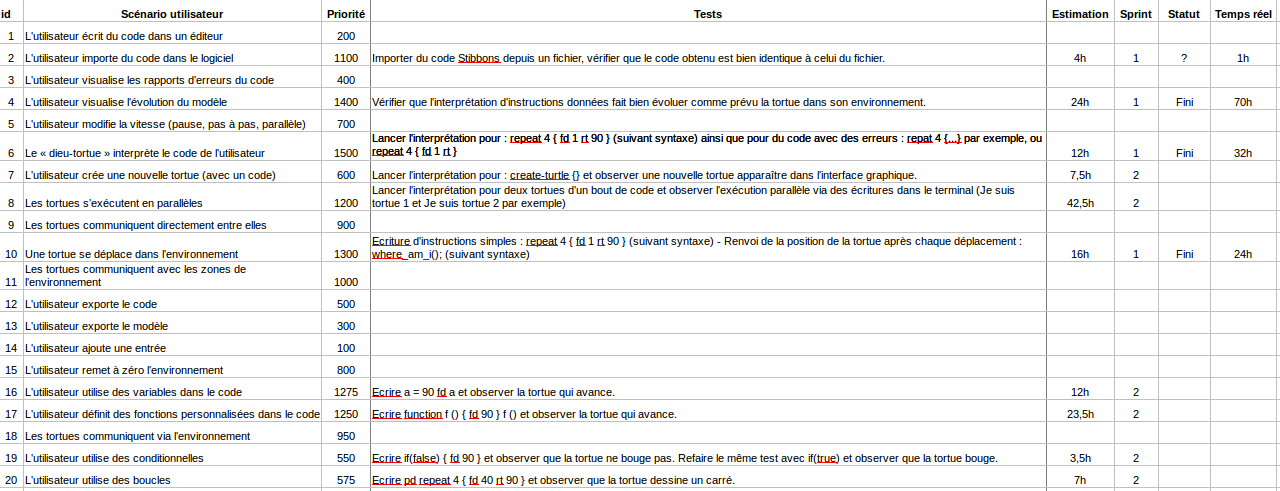
\includegraphics[scale=0.35]{doc/gestionProjet/backlogv1.png}
\end{figure}
